\documentclass{article}
\usepackage[utf8]{inputenc}
\usepackage[margin=1.5in]{geometry}
\usepackage[english]{babel}
\usepackage[dvipsnames]{xcolor}


% --- Figures ---
% \floatplacement{figure}{htb!} % (h)ere (t)op (b)ottom (p)age
\usepackage{graphicx}
\graphicspath{{figures/}}

\usepackage{subcaption}

% --- Math ---
\usepackage{amsmath}
\usepackage{nicefrac}

% --- Tables ---
\usepackage{booktabs}
\usepackage{csvsimple}

% --- Fonts ---
\usepackage{fontspec}
\usepackage[babel=true]{microtype}
\defaultfontfeatures{Ligatures=TeX}
\setmainfont{Source Serif Pro}[
  Path = fonts/source-serif-pro/SourceSerifPro-, Extension = .otf,
  Ligatures=TeX,
  UprightFont= Light,
  ItalicFont = LightIt,
  BoldFont   = Regular,
  BoldItalicFont = It]
\setsansfont{Roboto}[
  Ligatures=TeX,
  Path = fonts/roboto/Roboto-, Extension = .ttf,
  UprightFont = Light,
  ItalicFont = LightItalic,
  BoldFont = Regular]
\setmonofont{Source Code Pro}[
  Path = fonts/source-code-pro/SourceCodePro-, Extension = .otf,
  UprightFont = Light,
  BoldFont = Regular]

% --- Citations ---
\usepackage[style=apa,sortcites=true,sorting=nyt,backend=biber]{biblatex}
% TODO Following does not seem to work in subdirectory where it should be!
\addbibresource{tex/ref.bib}

% --- Header --- 

\title{A Careful Consideration of the St. Petersburg Paradox}
\author{Alexander R. Koen}
\date{\today}

\begin{document}
\maketitle

\section{The paradox}

If heads appears for the first time on turn $n$, the player is awarded $\$2^n$.


\begin{align*}
\label{eq:1}
  EMV &= \sum_{n=1}^{\infty} \frac{1}{2^{n}}2^n \\
      &= \sum_{n=1}^{\infty}1 \\
      &= \infty
\end{align*}

The St. Petersburg game's possible winnings are geometrically distributed with $Pr(n)=\frac{1}{2}^{n}$, where $Pr(n)$ is the probability of toss $n$ being the first occurrence of heads and thus winning $\$2^n$.

\begin{figure}[htb]
  \centering
  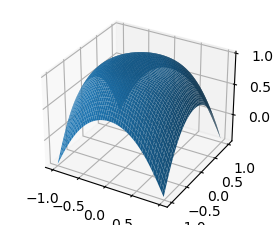
\includegraphics{distribution}
  \caption{Distribution of payouts in one round of the St. Petersburg Game. Each bar has an area of 1 and thus the expected value is infinite.}
  \label{fig:distribution}
\end{figure}

\section{Simulating for world}

\begin{table}[htb]
  \centering
  \begin{tabular}{cc}
    \toprule
    \textbf{Winnings ($\$2^n$)} & \textbf{Number of People} \\
    \midrule
    1 & 5022 \\
2 & 2521 \\
3 & 1255 \\
4 & 609 \\
5 & 314 \\
6 & 142 \\
7 & 68 \\
8 & 34 \\
9 & 15 \\
10 & 11 \\
11 & 5 \\
12 & 3 \\
13 & 1 \\
14 & 0 \\
15 & 0 \\
16 & 0 \\
17 & 0 \\
    \bottomrule
  \end{tabular}
  \caption{World}
  \label{tab:world}
\end{table}


\begin{figure}[htb]
  \centering
  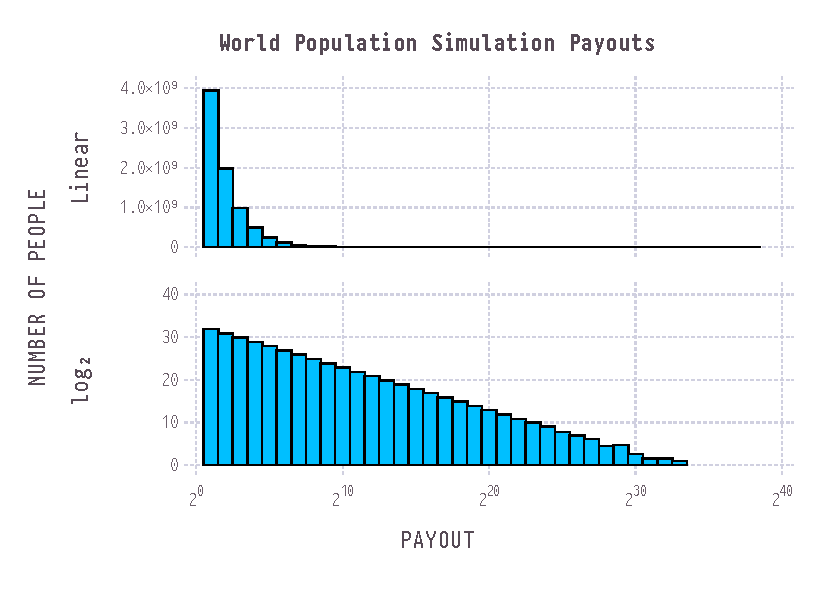
\includegraphics{world}
  \caption{Change}
  \label{fig:distribution}
\end{figure}

\section{Lottery}

\begin{table}[htb]
  \centering
  \begin{tabular}{cc}
    \toprule
    \textbf{Winnings ($\$2^n$)} & \textbf{Number of People} \\
    \midrule
    $150,000,000$ & $1:292,291,338$\\
    \bottomrule
  \end{tabular}
  \caption{Lottery}
  \label{tab:lotto}
\end{table}

\section{Evolution}

\begin{figure}[htb]
  \centering
  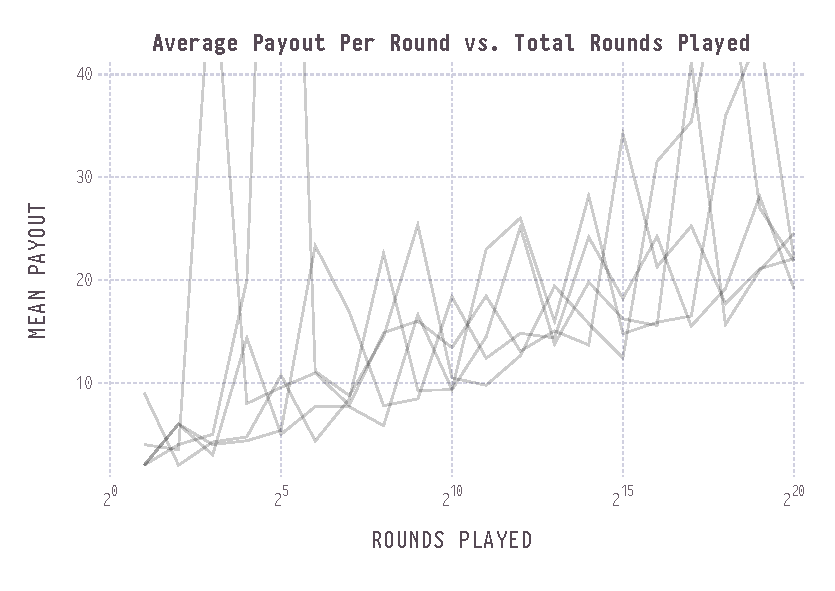
\includegraphics[width=\textwidth]{average-over-time}
  \caption{Payout}
\end{figure}

\begin{figure}[htb]
  \centering
  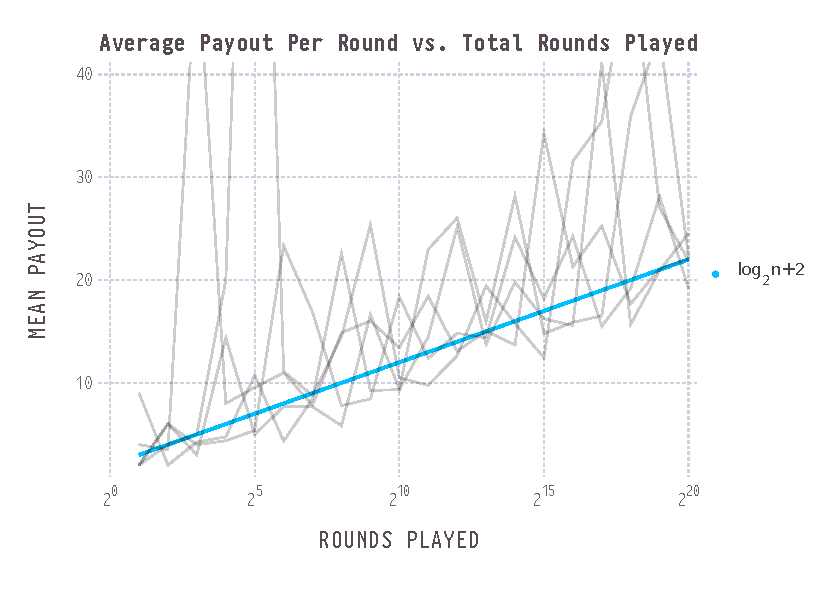
\includegraphics[width=\textwidth]{average-over-time-fit}
  \caption{Payout Fit}
\end{figure}

\begin{figure}[htb]
  \centering
  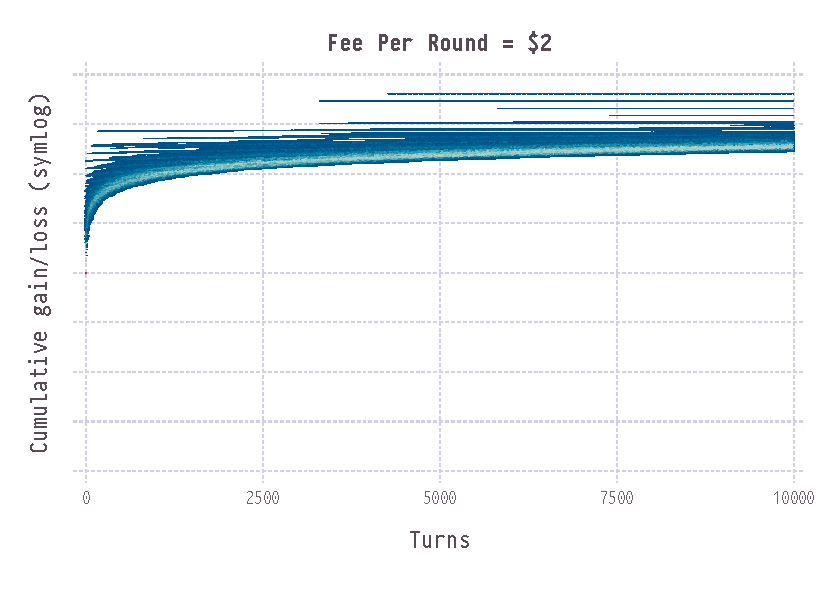
\includegraphics[width=\textwidth]{winnings-2}
  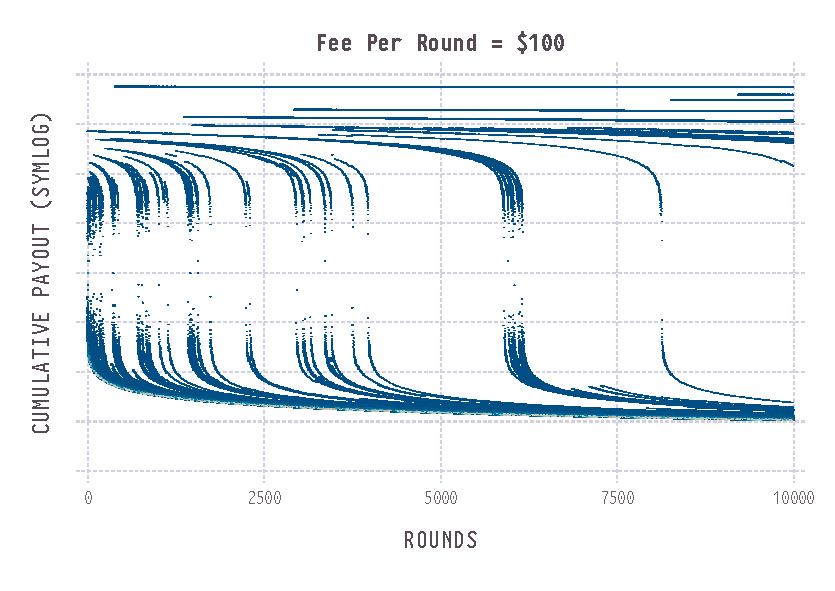
\includegraphics[width=\textwidth]{winnings-100}
  
  \caption{With a per-round fee of \$2, the player wins every time. If that fee is increased to a hundred dollars, however, most players will suffer a loss after 10,000 rounds.}
  \label{fig:evolution}
\end{figure}\label{fig:payout_p}

\begin{minipage}{\textwidth}
\section{Steinhaus Sequence}
Start with an empty sequence of infinite length. Now fill every \textit{other} element with a 2.

\[\begin{bmatrix}{\color{RawSienna} 2} & \_ & {\color{RawSienna} 2} & \_ & {\color{RawSienna} 2} & \_ & {\color{RawSienna} 2}\dots\end{bmatrix} \]

{Fill every 4th\textsuperscript{th} element with a 4.

\[\begin{bmatrix}2 & {\color{RawSienna} 4} & 2 & \_ & 2 & {\color{RawSienna} 4} & 2\dots\end{bmatrix} \]

Fill every 8th\textsuperscript{th} element with an 8.

\[\begin{bmatrix}2 & 4 & 2 & {\color{RawSienna} 8} & 2 & 4 & 2\dots\end{bmatrix} \]

And so on\dots\\\\
\end{minipage}

This approach was first proposed by \textcite{Steinhaus1949}.
  

Notice that this represents exactly expected payouts of the St. Petersburg Game. Picking randomly from elements in the sequence will produce 2 half the time, 4 one-quarter of the time, 8 one-eight of the time, and so forth.

One can therefore reformulate the paradox as a random draw



When the per-round fee is set to $\log_2N+2$, where $N$ is the total number of rounds played, wealth is asymptotically stable as shown in Figure \ref{fig:evolution-fair}. Note that on most rounds the player will lose money, but this is offset by the occasional large payout from the house.

\begin{figure}[htb]
  \centering
  \includegraphics[width=\textwidth]{winnings-N}
    \caption{Evolution of gain/loss over 10,000 round with a per-round fee of $\log_2(10000)+2$. As expected, with this fee wealth is asymptotically stable.}
    \label{fig:evolution-fair}
  \end{figure}

\clearpage
\printbibliography
\end{document}
